\section{Windows}
\subsection{Attribution des paramètres réseaux}

Démarrer la machine virtuelle Windows 10. Accéder aux paramètres réseau et Internet, en cliquant droit sur l'icône de réseau sur la droite de la barre des tâches. Cliquer sur \textit{Ouvrir les paramètres réseau et Internet} :
\begin{figure}[h!]
	\begin{center}
		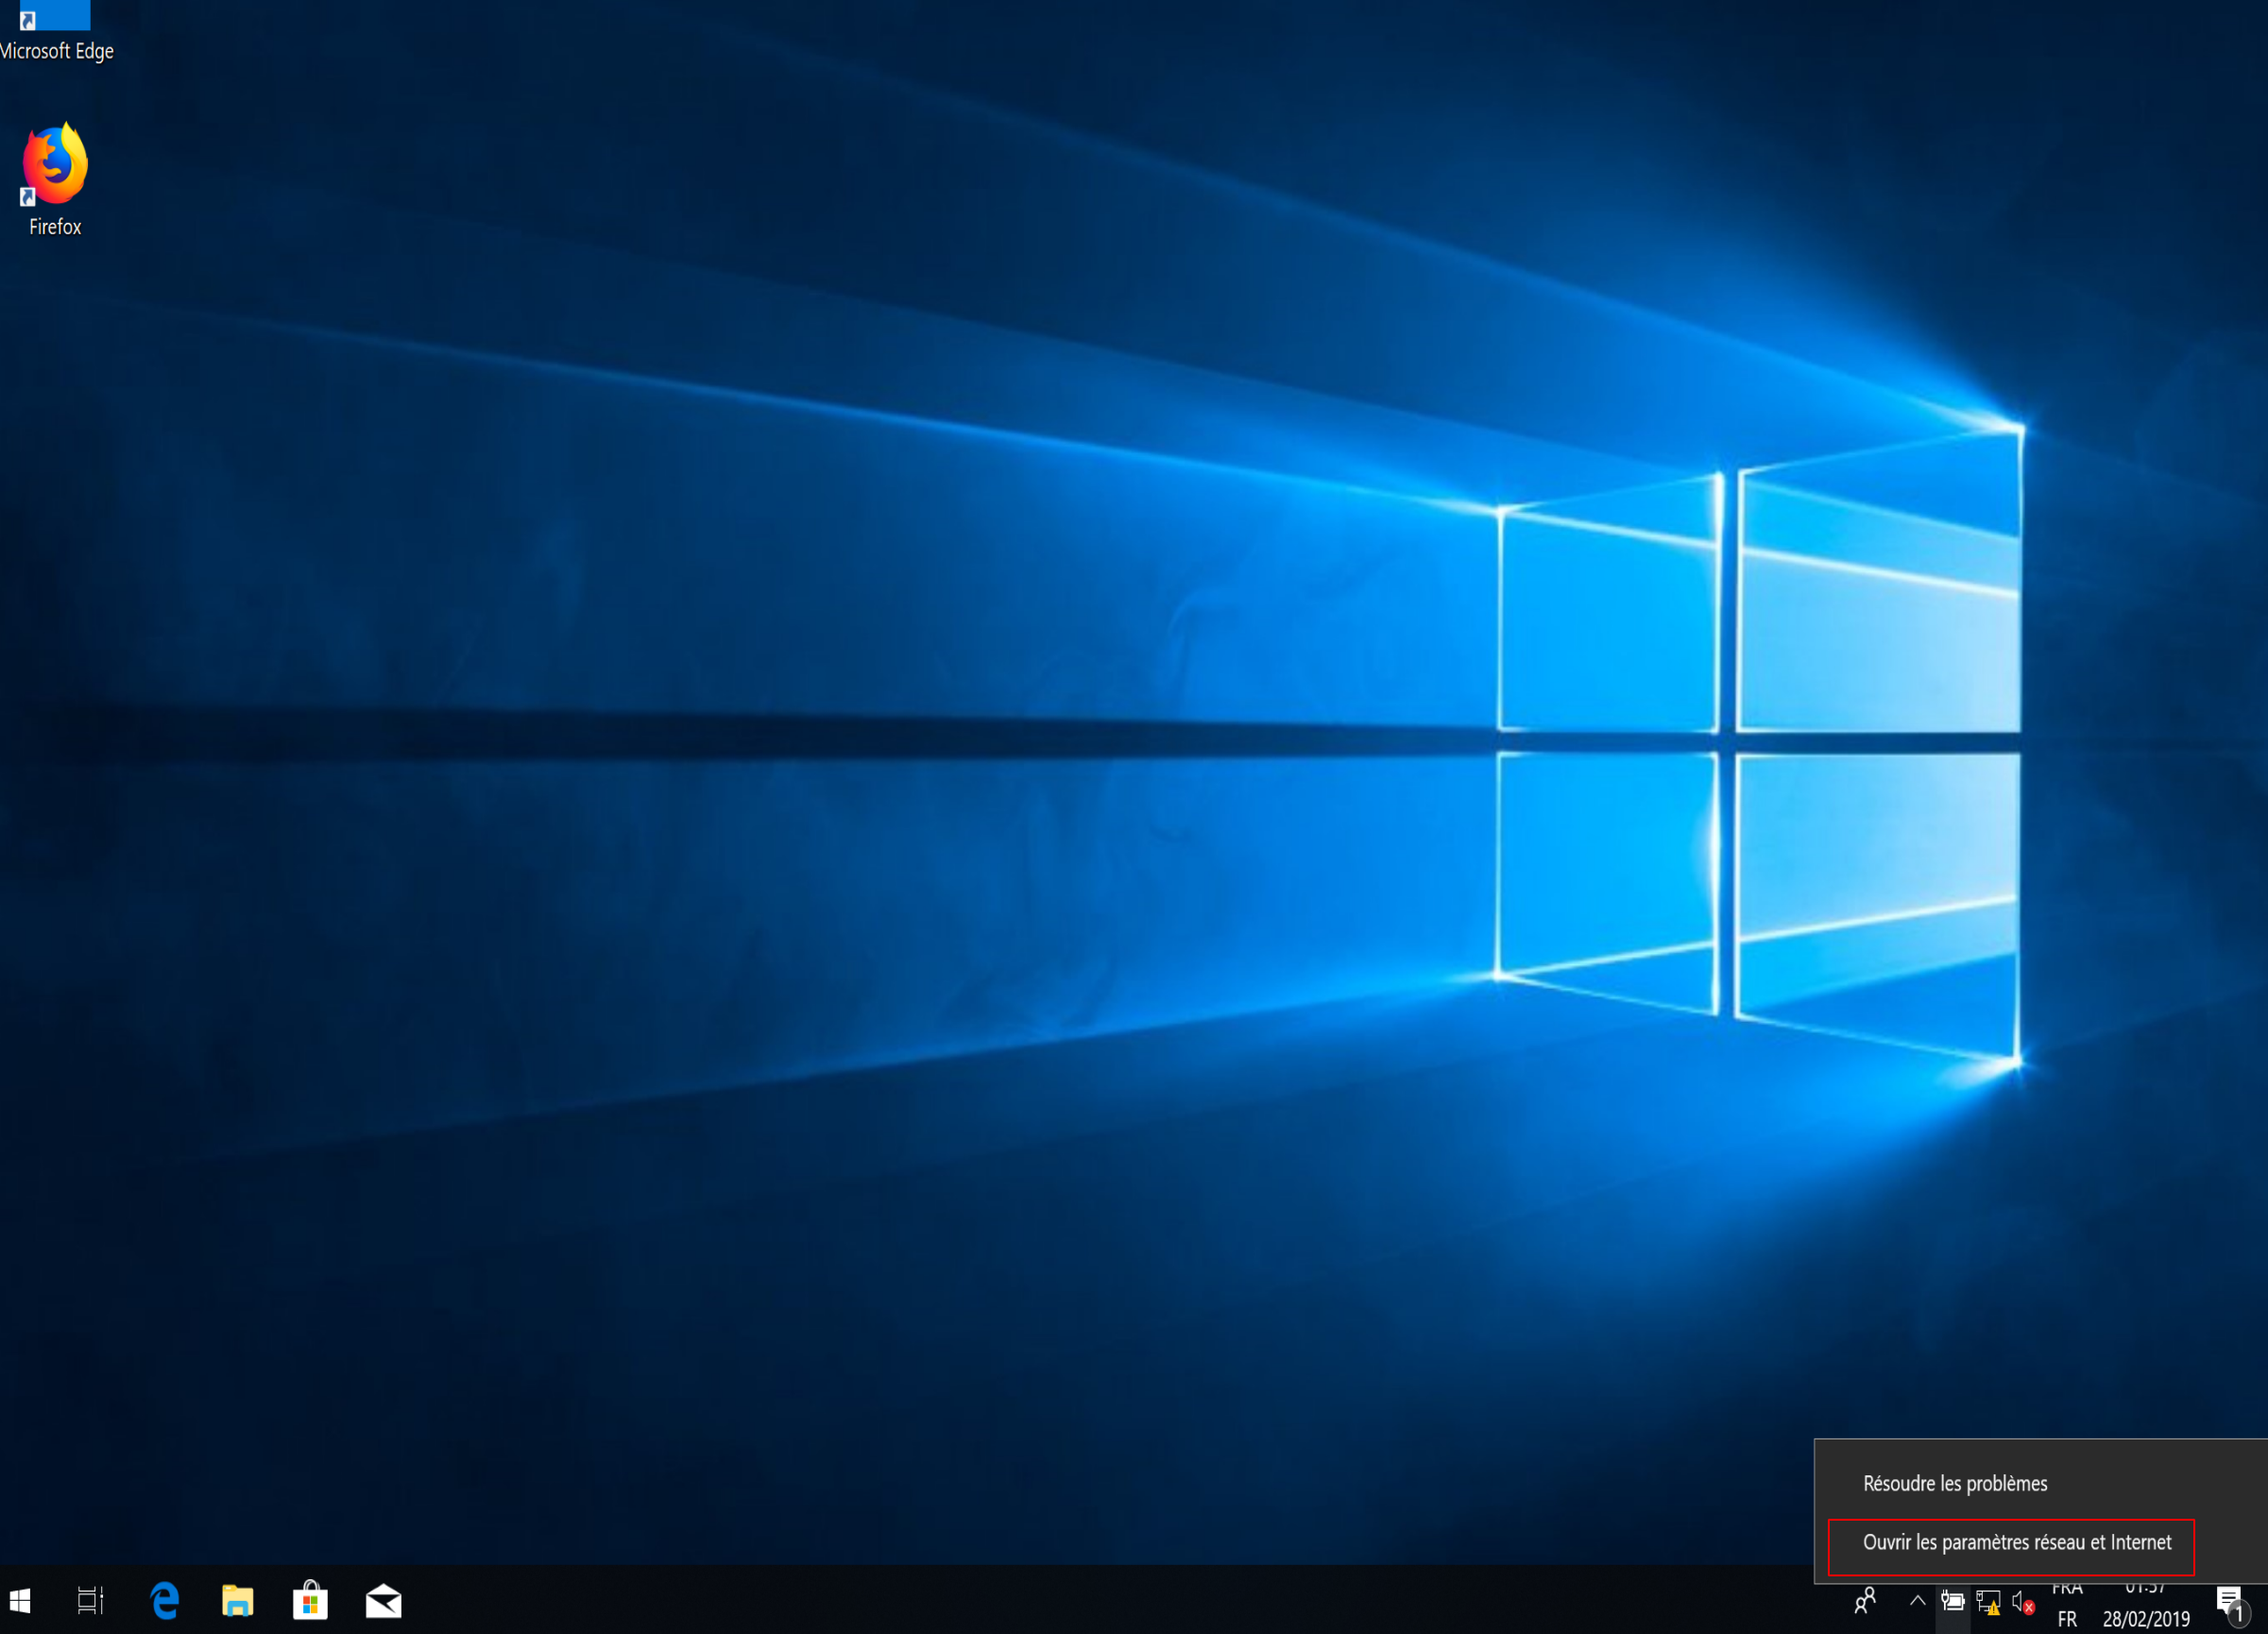
\includegraphics[scale=0.6]{W_Screenshots/41.png}
		\caption{Accès aux paramètres réseau et Internet de Windows 10}
		\label{W_Screenshots/41}
	\end{center}
\end{figure}
\FloatBarrier

\newpage
Ouvrir les options d'adaptateur, en cliquant sur \textit{Modifier les options d'adapteur} :
\begin{figure}[h!]
	\begin{center}
		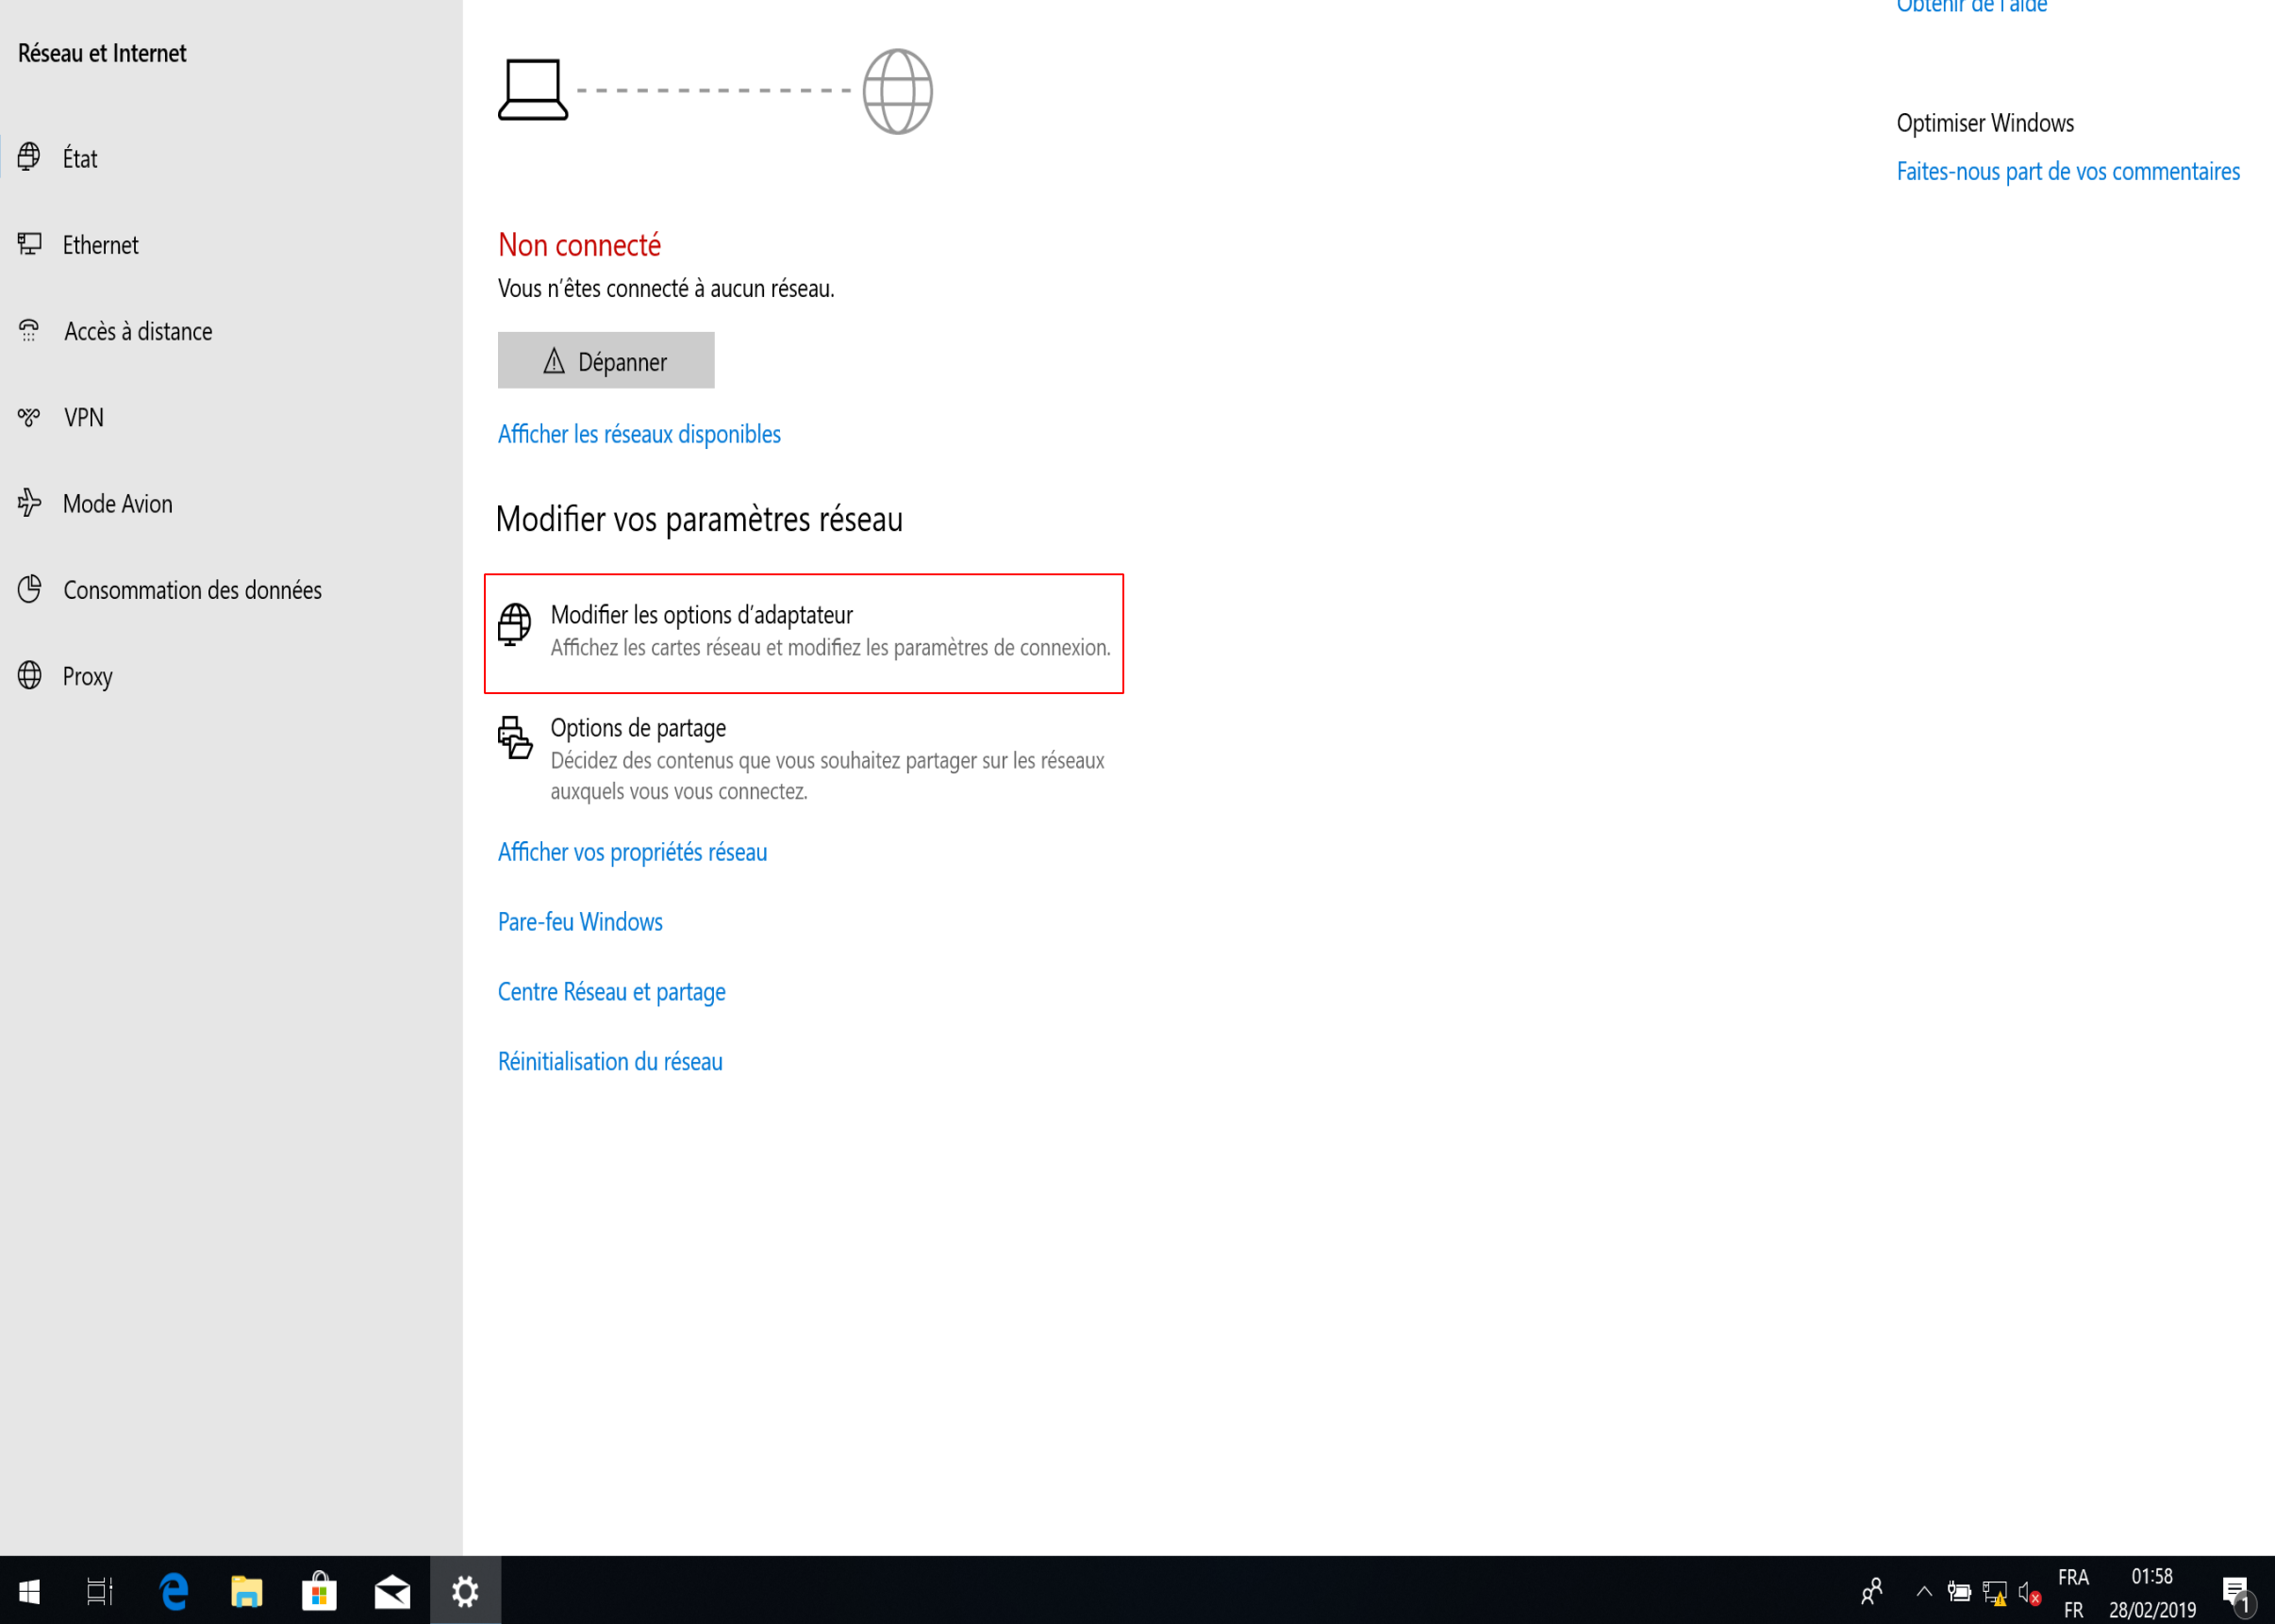
\includegraphics[scale=0.6]{W_Screenshots/42.png}
		\caption{Ouverture des options d'adaptateur de Windows 10}
		\label{W_Screenshots/42}
	\end{center}
\end{figure}
\FloatBarrier

\newpage
Cliquer droit sur la carte Ethernet, et sélectionner \textit{Propriétés} :
\begin{figure}[h!]
	\begin{center}
		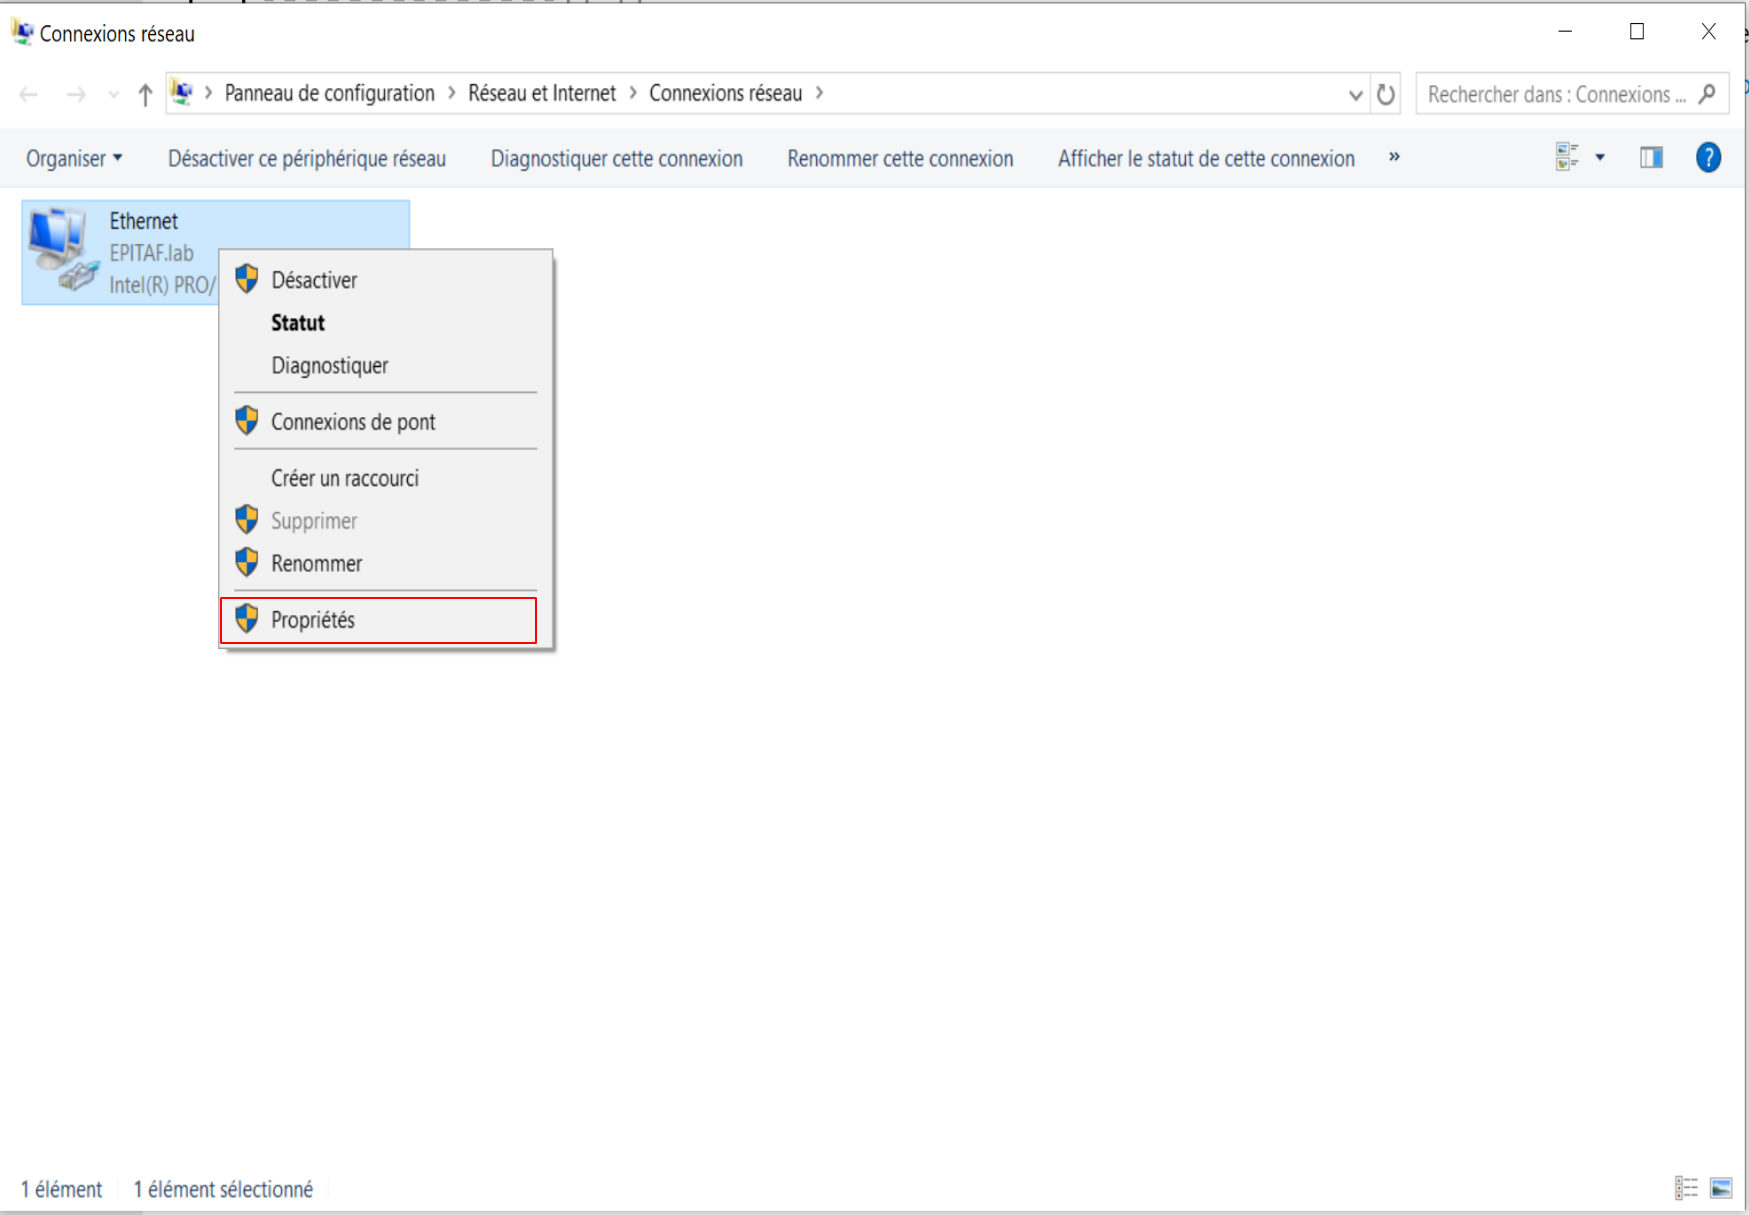
\includegraphics[scale=0.8]{W_Screenshots/43.png}
		\caption{Accès aux propriétés de la carte Ethernet de Windows 10}
		\label{W_Screenshots/43}
	\end{center}
\end{figure}
\FloatBarrier

\newpage
Décocher \textit{Protocole Internet version 6 (TCP/IPv6)}, et cocher \textit{Protocole Internet version 4 (TCP/IPv4)}. Cliquer sur \textit{Propriétés} pour IPv4 :
\begin{figure}[h!]
	\begin{center}
		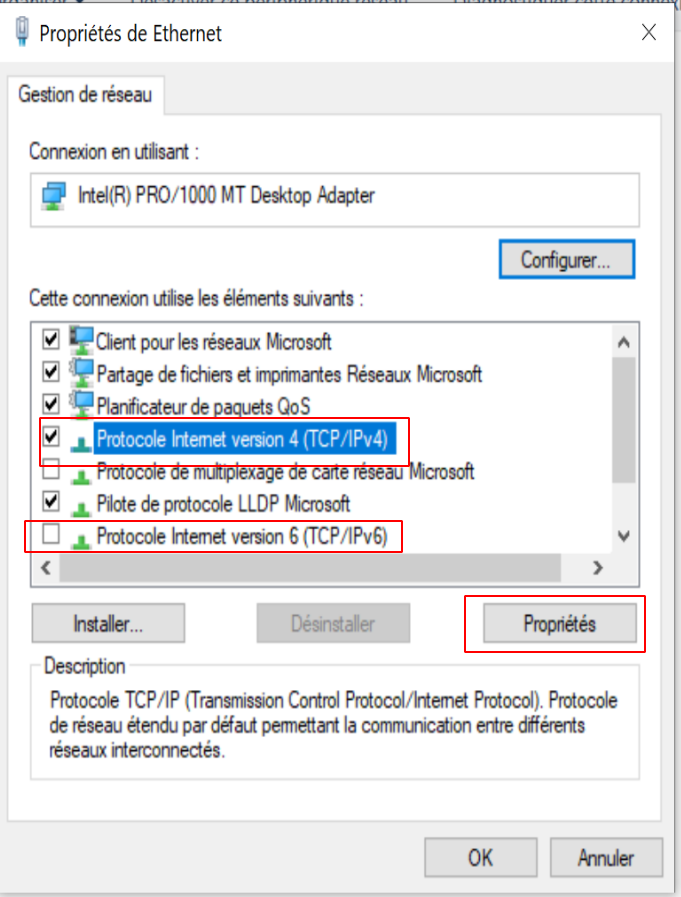
\includegraphics[scale=0.8]{W_Screenshots/44.png}
		\caption{Modification sur les protocoles Internet et accès aux propriétés IPv4 de Windows 10}
		\label{W_Screenshots/44}
	\end{center}
\end{figure}
\FloatBarrier

Renseigner la valeur du serveur DNS préféré : 192.168.2.2. Cliquer sur \textit{OK} :
\begin{figure}[h!]
	\begin{center}
		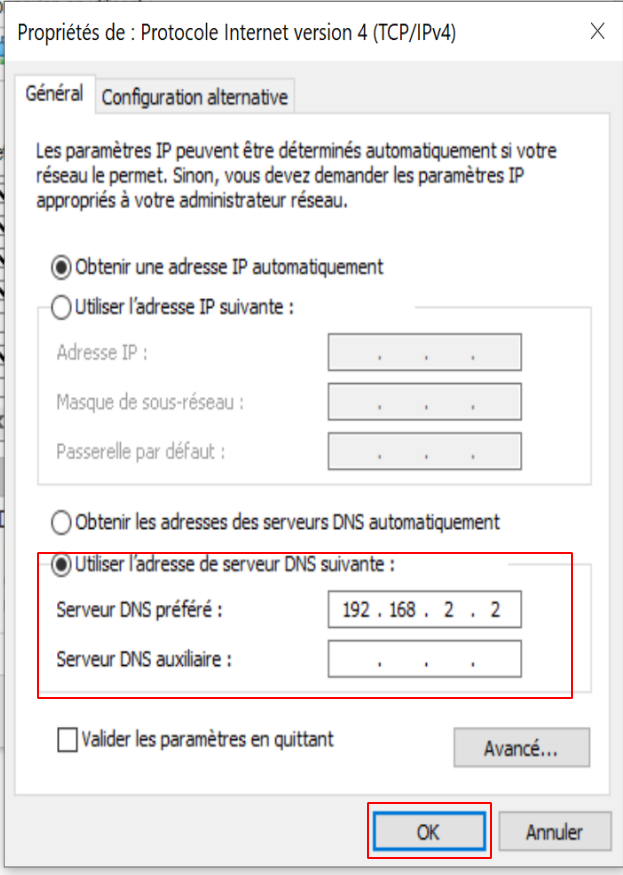
\includegraphics[scale=0.8]{W_Screenshots/45.png}
		\caption{Modification de l'adresse DNS de PC01 de Windows 10}
		\label{W_Screenshots/45}
	\end{center}
\end{figure}
\FloatBarrier 
    
\subsection{Attribution du domaine}

Accéder aux paramètres \textit{Systèmes} :
\begin{figure}[h!]
	\begin{center}
		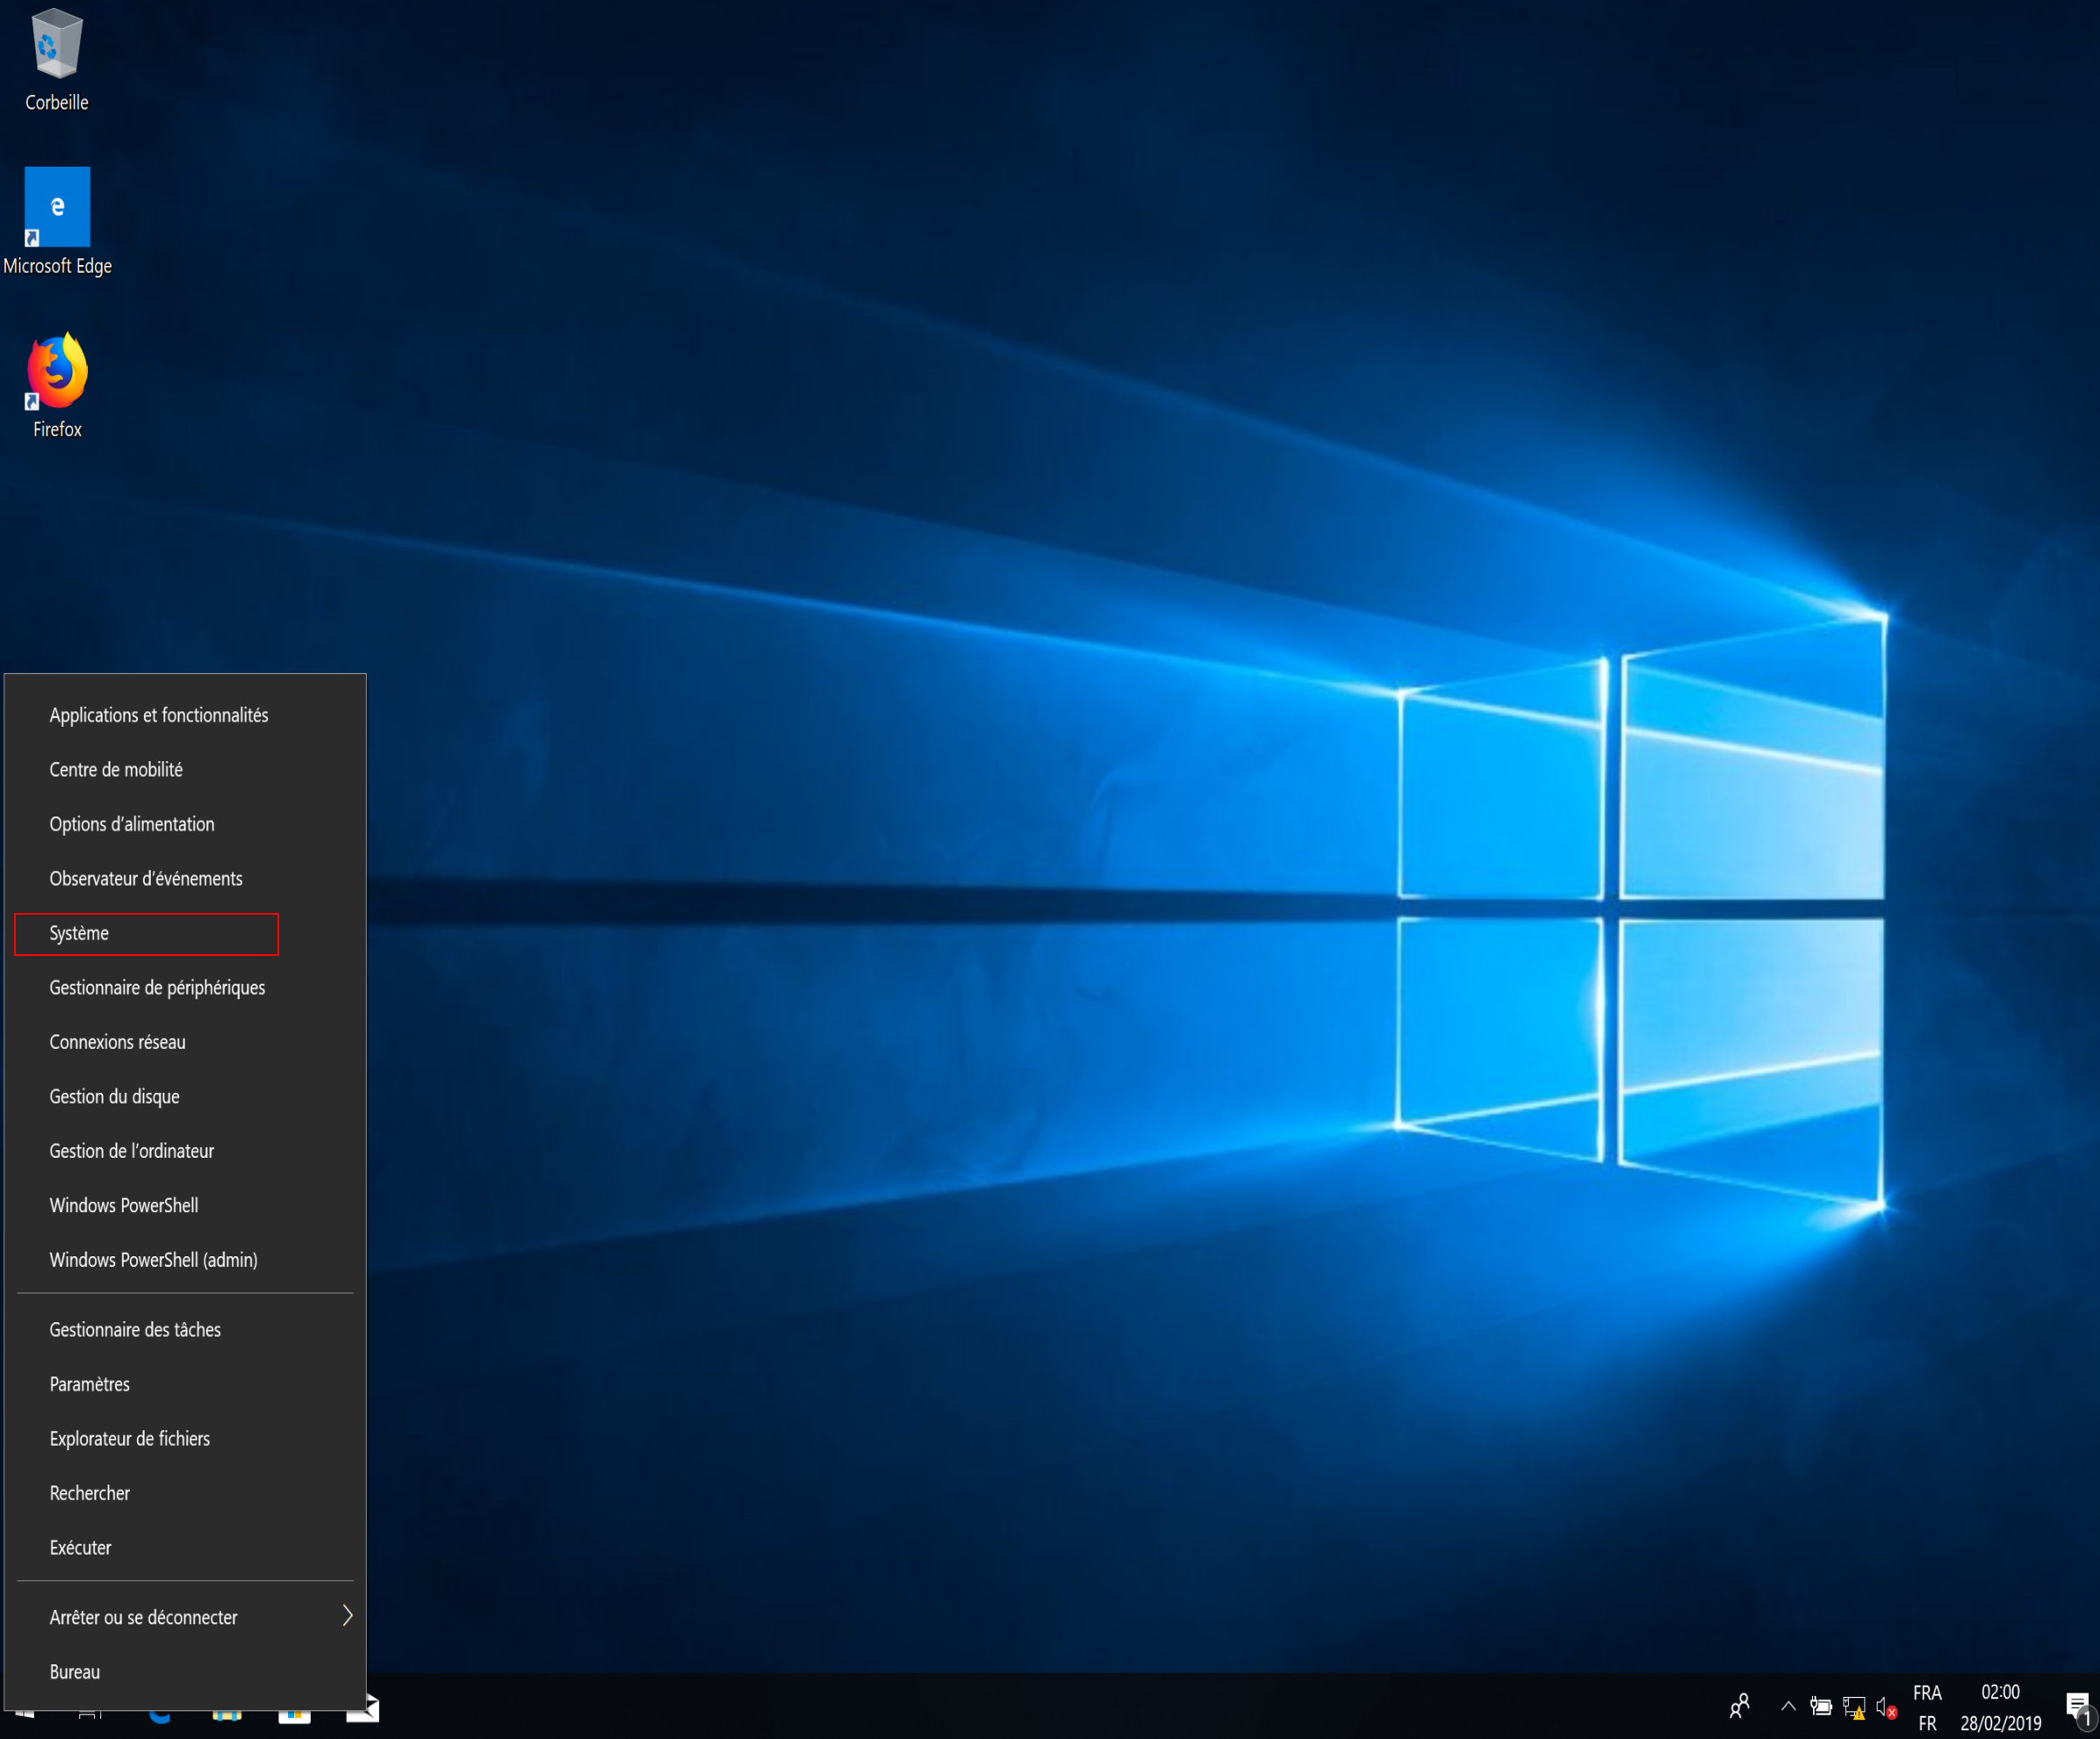
\includegraphics[scale=0.6]{W_Screenshots/46.png}
		\caption{Accès à Système sur Windows 10}
		\label{W_Screenshots/46}
	\end{center}
\end{figure}
\FloatBarrier

\newpage
Aller à la section \textbf{Informations Système}. Cliquer sur \textit{Informations système} :
\begin{figure}[h!]
	\begin{center}
		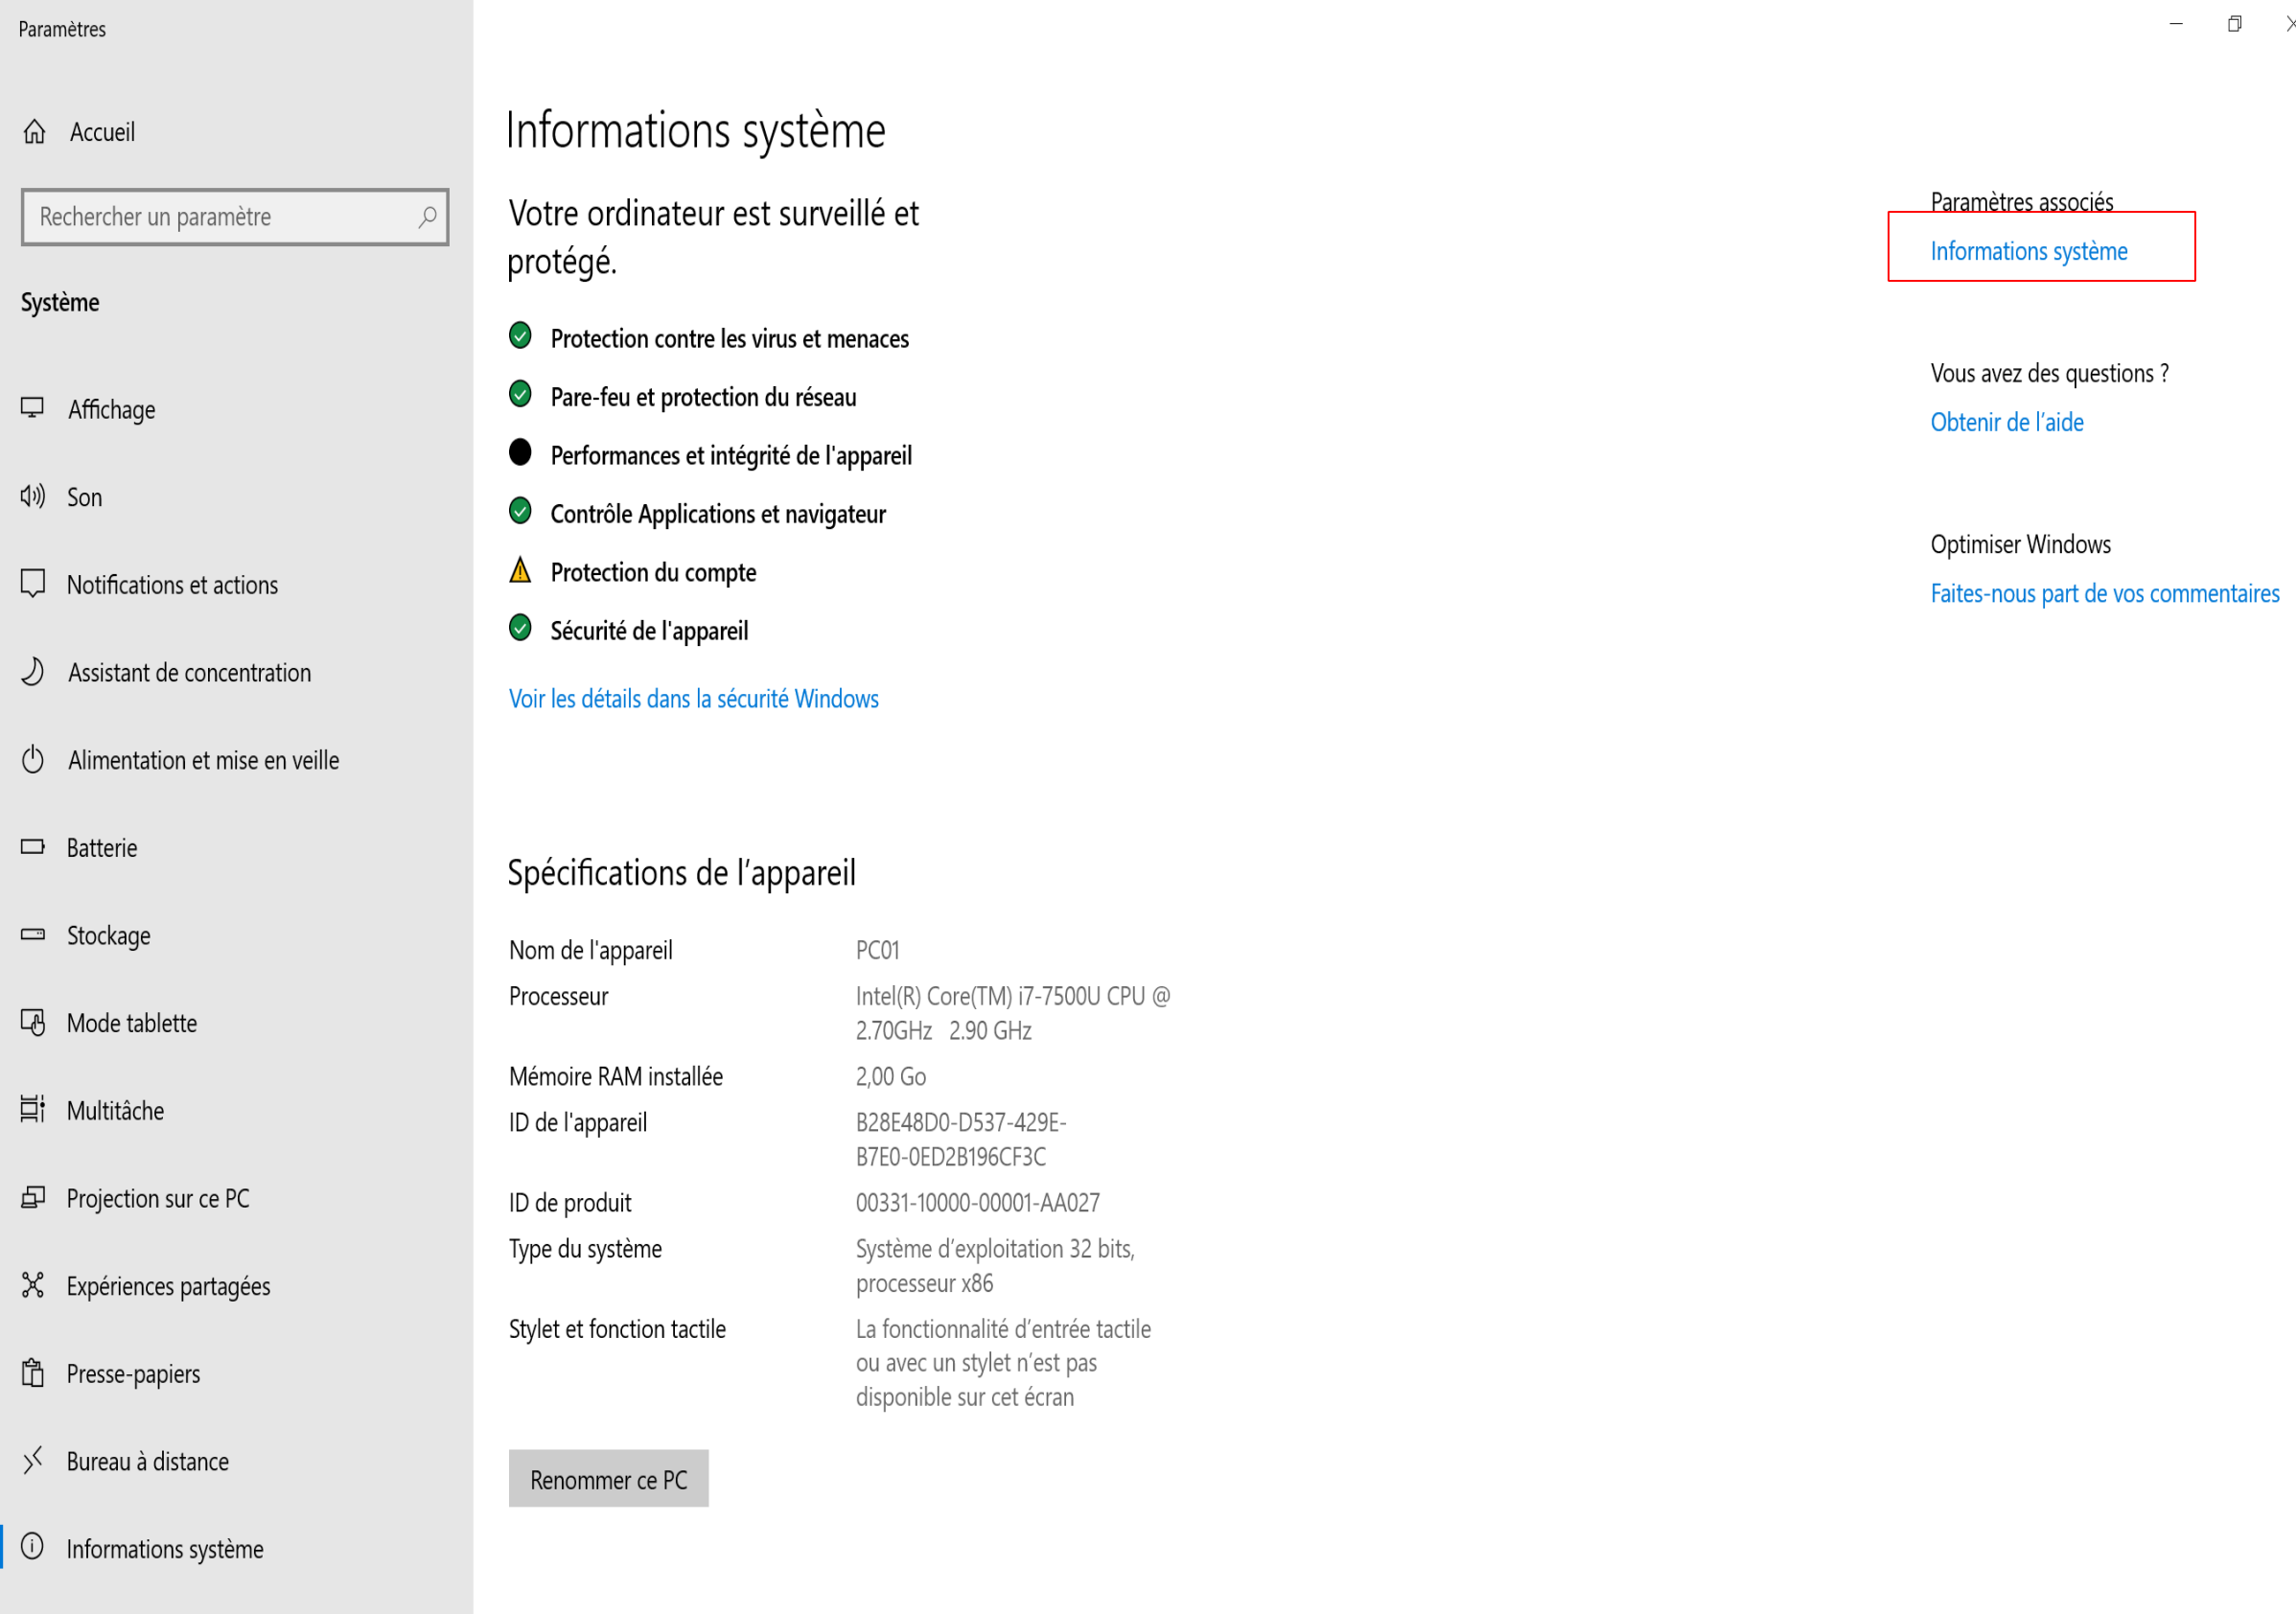
\includegraphics[scale=0.6]{W_Screenshots/47.png}
		\caption{Accès à Informations Système de Windows 10}
		\label{W_Screenshots/47}
	\end{center}
\end{figure}
\FloatBarrier

\newpage
Cliquer sur \textit{Modifier les paramètres} :
\begin{figure}[h!]
	\begin{center}
		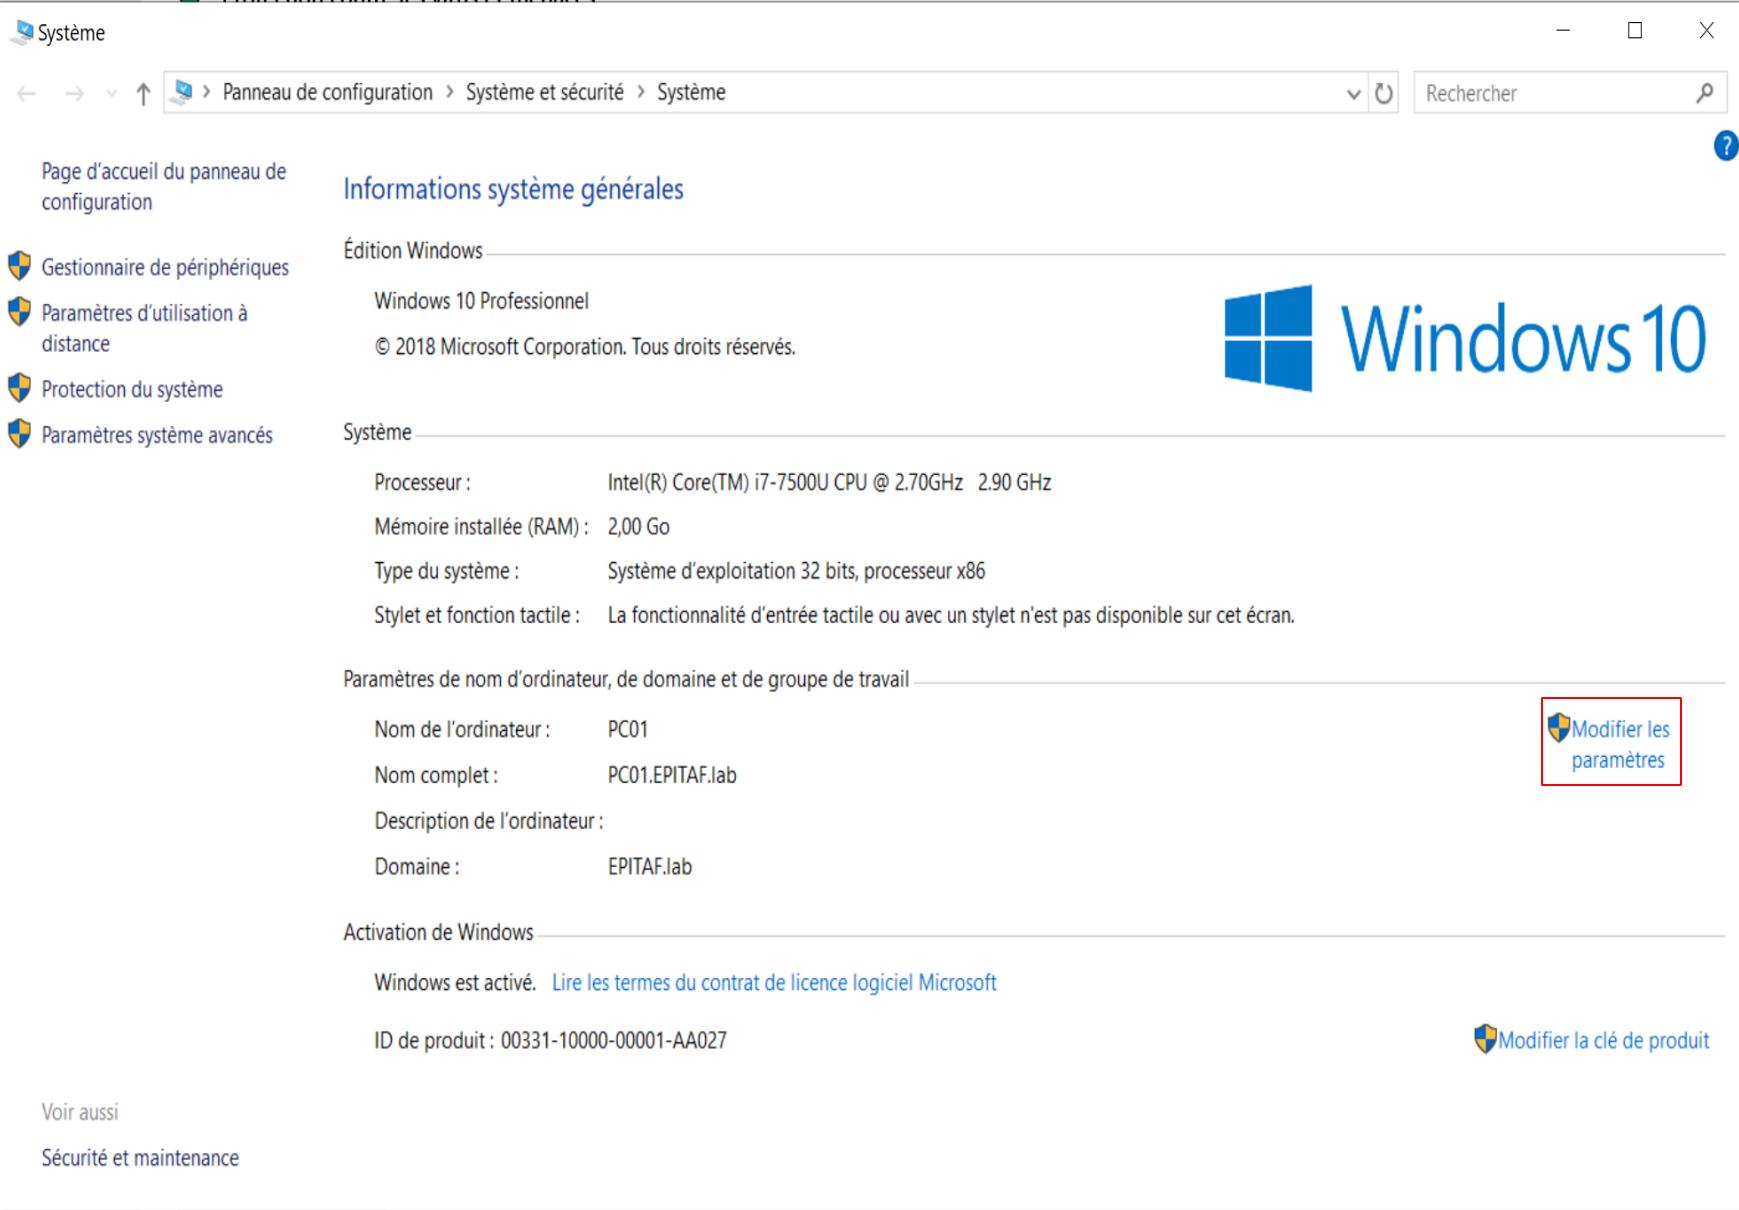
\includegraphics[scale=0.7]{W_Screenshots/48.png}
		\caption{Accès à la modification des paramètres système de Windows 10}
		\label{W_Screenshots/48}
	\end{center}
\end{figure}
\FloatBarrier

\newpage
Accéder aux propriétés de domaine en cliquant sur \textit{Modifier} :
\begin{figure}[h!]
	\begin{center}
		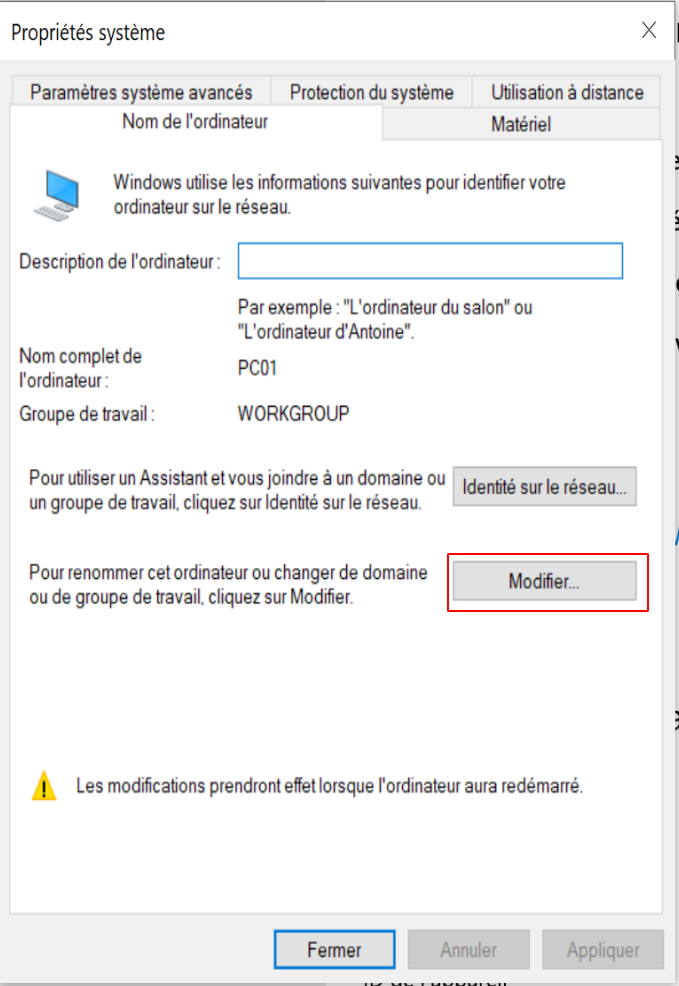
\includegraphics[scale=1]{W_Screenshots/49.png}
		\caption{Accès aux propriétés de domaine de Windows 10}
		\label{W_Screenshots/49}
	\end{center}
\end{figure}
\FloatBarrier

\newpage
Ajouter le domaine \textbf{EPITAF}, et cliquer sur \textit{OK} :
\begin{figure}[h!]
	\begin{center}
		\includegraphics[scale=0.22]{PC01/PC11.png}
		\caption{Modification du domaine de Windows 10}
		\label{W_Screenshots/50}
	\end{center}
\end{figure}
\FloatBarrier

\newpage
Rentrer les identifiants demandés, par exemple :
\begin{itemize}
    \item \textit{Nom d'utilisateur} : EPITAF\textbackslash Ultrae;
    \item \textit{Mot de passe} : celui associé à Ultrae.
\end{itemize}
Un message de bienvenue apparaît si les identifiants sont corrects. Cliquer sur \textit{OK} puis fermer toutes les fenêtres :
\begin{figure}[h!]
	\begin{center}
		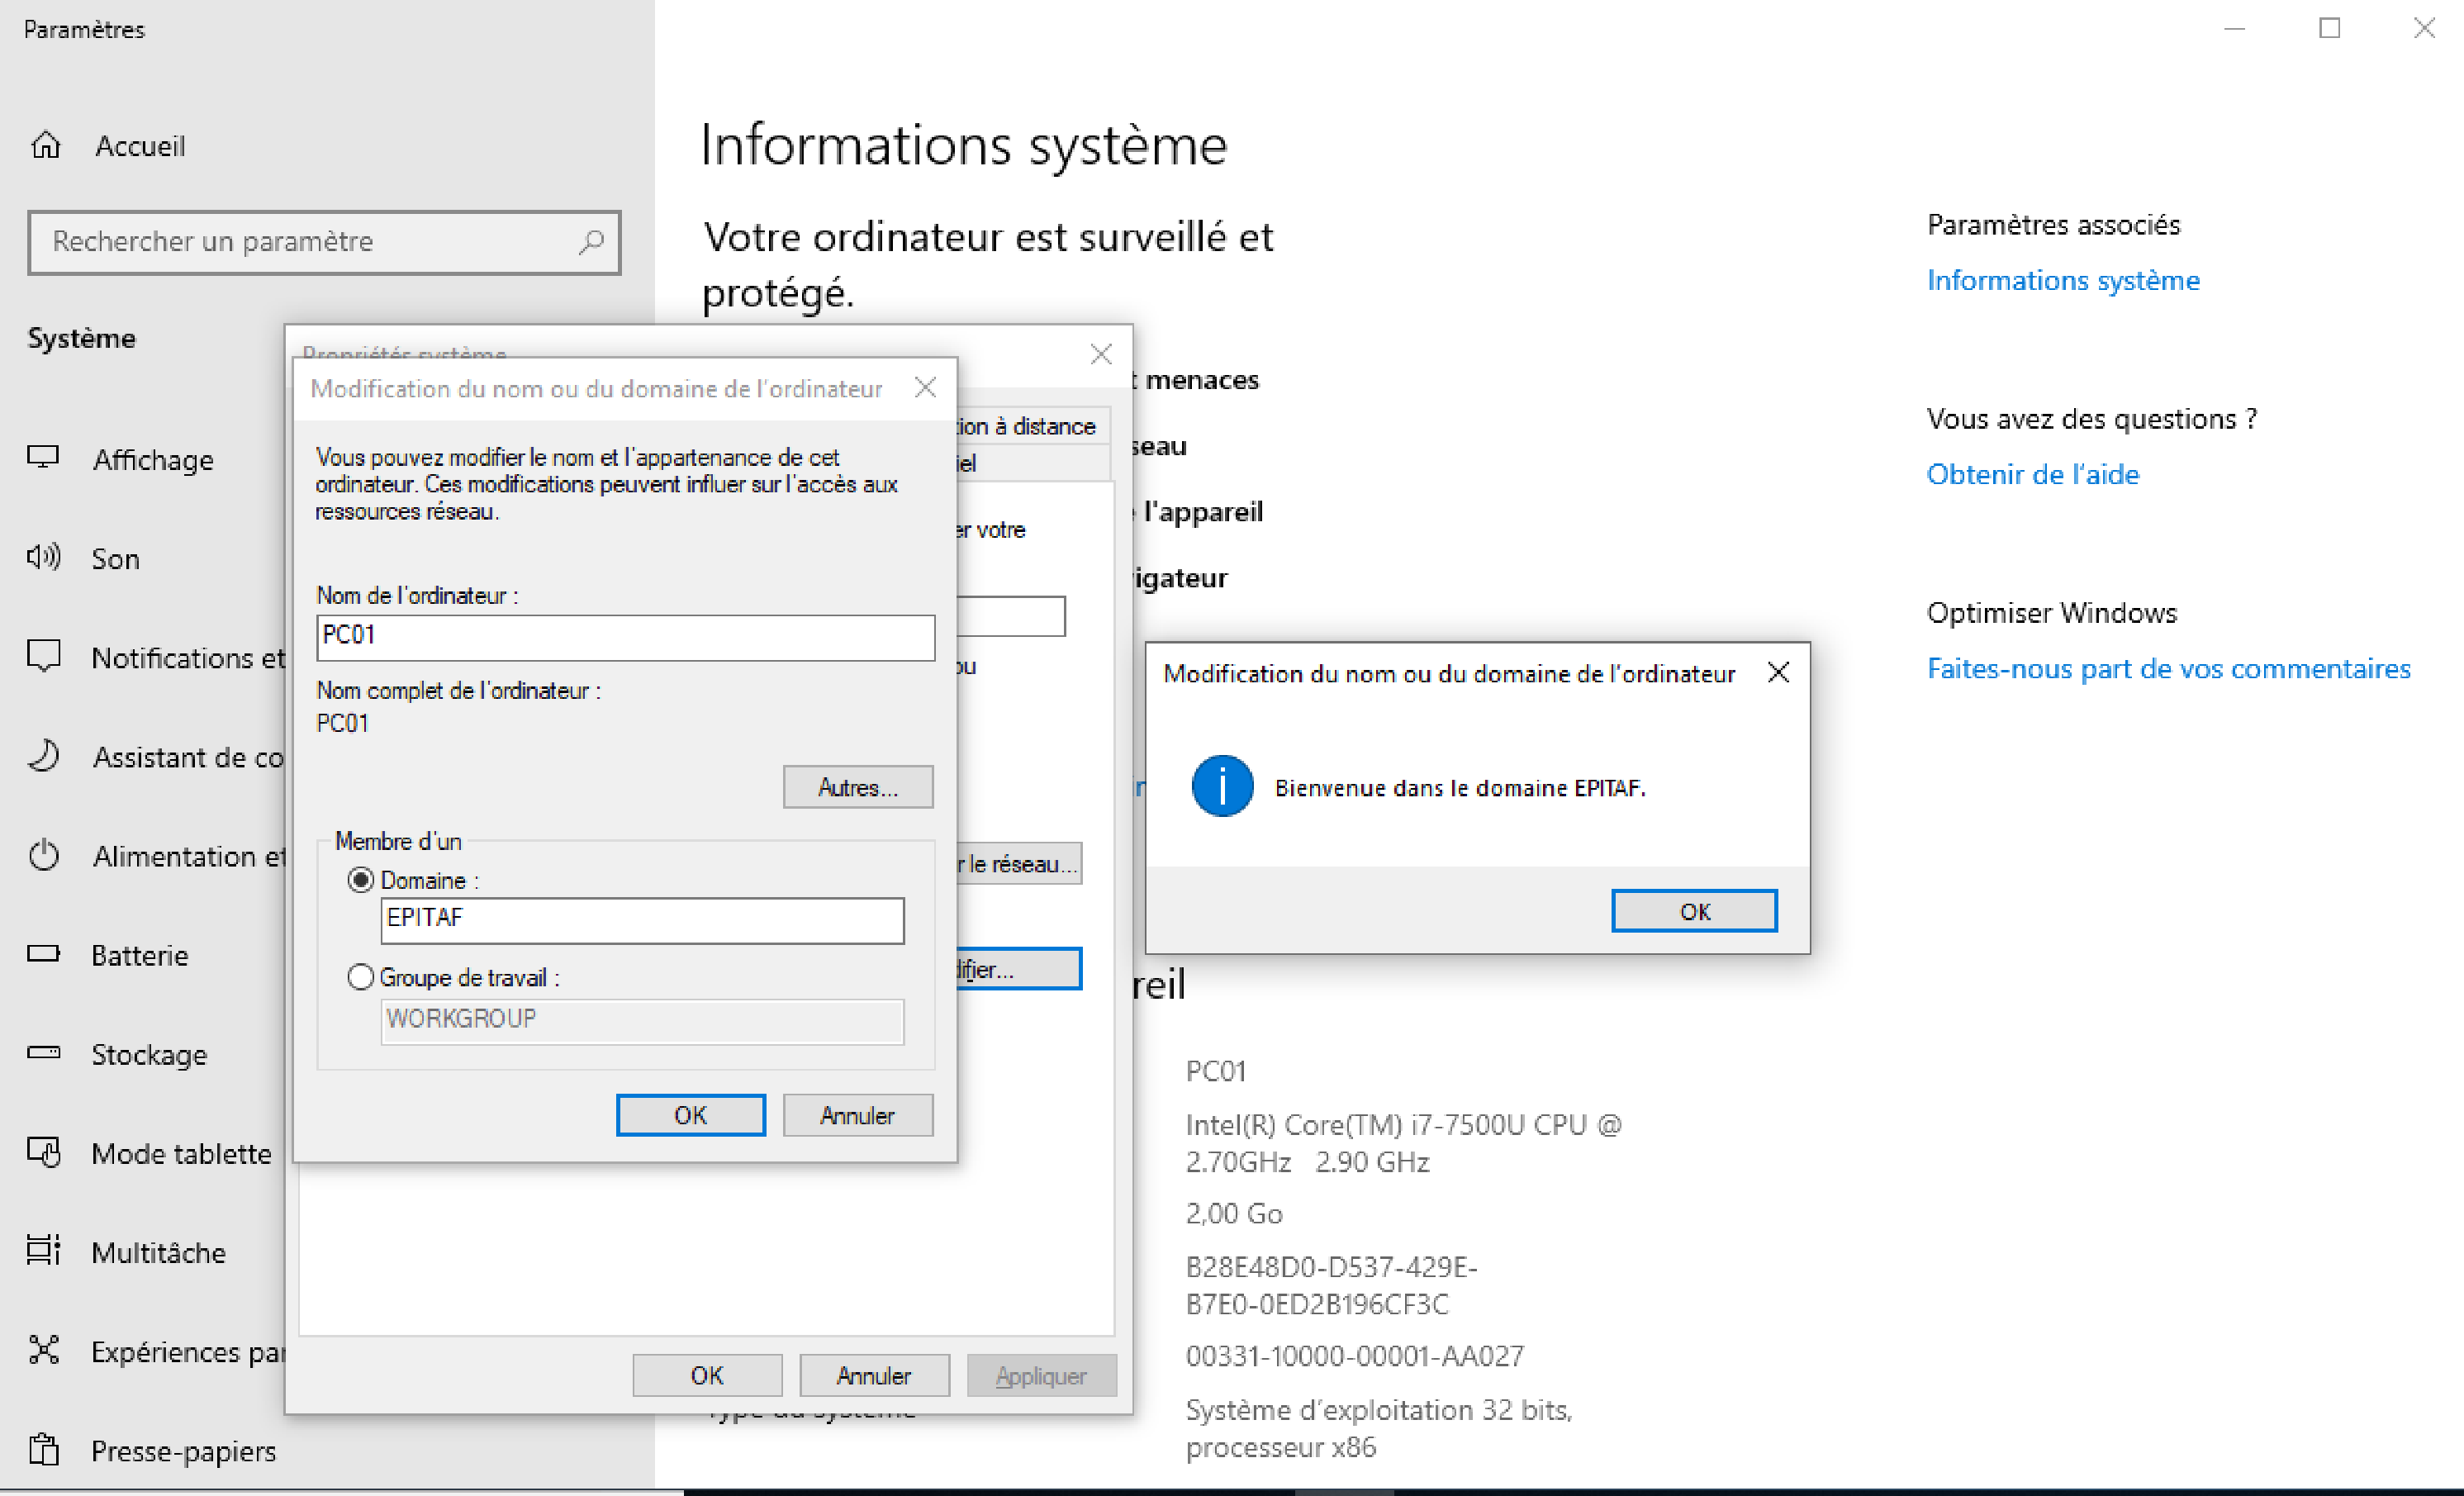
\includegraphics[scale=0.5]{W_Screenshots/51.png}
		\caption{Modification de domaine effective de Windows 10}
		\label{W_Screenshots/51}
	\end{center}
\end{figure}
\FloatBarrier